\documentclass{standalone}
\usepackage{tikz}
\usetikzlibrary{patterns, positioning}

\begin{document}
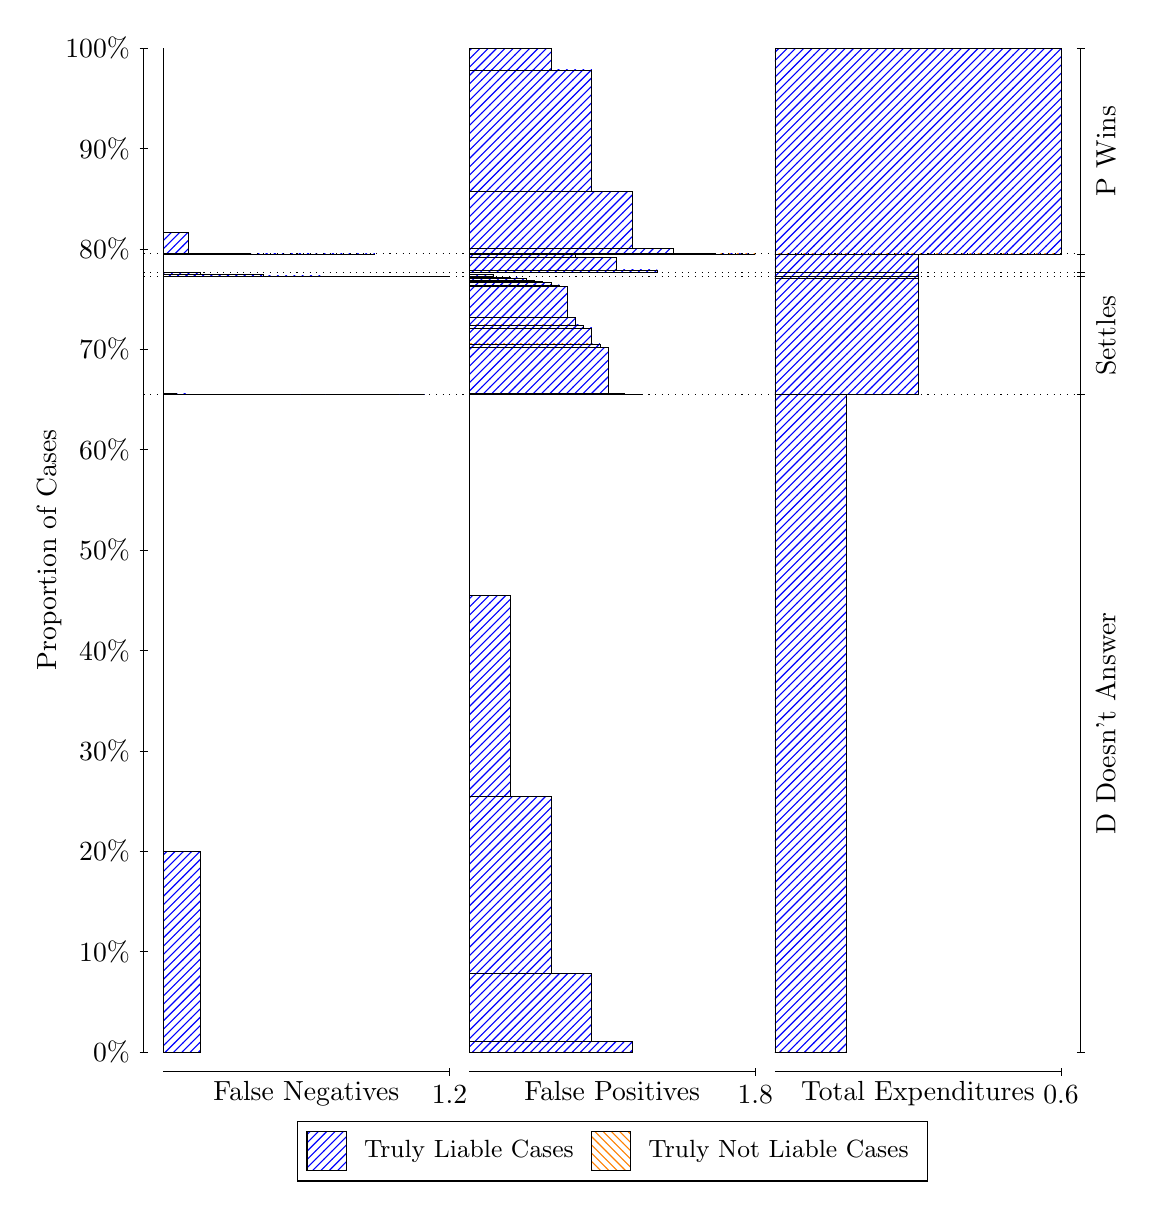
\begin{tikzpicture}
\draw[black, very thin] (1.5,1.75) -- (1.5,14.5);
\node[rotate=90, anchor=center] at (0.3, 8.125) {Proportion of Cases};
\draw[black, very thin] (1.45,1.75) -- (1.55,1.75);
\node[anchor=east] at (1.45, 1.75) {0\%};
\draw[black, very thin] (1.45,3.025) -- (1.55,3.025);
\node[anchor=east] at (1.45, 3.025) {10\%};
\draw[black, very thin] (1.45,4.3) -- (1.55,4.3);
\node[anchor=east] at (1.45, 4.3) {20\%};
\draw[black, very thin] (1.45,5.575) -- (1.55,5.575);
\node[anchor=east] at (1.45, 5.575) {30\%};
\draw[black, very thin] (1.45,6.85) -- (1.55,6.85);
\node[anchor=east] at (1.45, 6.85) {40\%};
\draw[black, very thin] (1.45,8.125) -- (1.55,8.125);
\node[anchor=east] at (1.45, 8.125) {50\%};
\draw[black, very thin] (1.45,9.4) -- (1.55,9.4);
\node[anchor=east] at (1.45, 9.4) {60\%};
\draw[black, very thin] (1.45,10.675) -- (1.55,10.675);
\node[anchor=east] at (1.45, 10.675) {70\%};
\draw[black, very thin] (1.45,11.95) -- (1.55,11.95);
\node[anchor=east] at (1.45, 11.95) {80\%};
\draw[black, very thin] (1.45,13.225) -- (1.55,13.225);
\node[anchor=east] at (1.45, 13.225) {90\%};
\draw[black, very thin] (1.45,14.5) -- (1.55,14.5);
\node[anchor=east] at (1.45, 14.5) {100\%};

\draw[black, very thin] (13.4,1.75) -- (13.4,14.5);
\draw[black, very thin] (13.35,1.75) -- (13.45,1.75);
\node[anchor=west] at (13.35, 1.75) {};
\draw[black, very thin] (13.35,10.097) -- (13.45,10.097);
\node[anchor=west] at (13.35, 10.097) {};
\draw[black, very thin] (13.35,11.597) -- (13.45,11.597);
\node[anchor=west] at (13.35, 11.597) {};
\draw[black, very thin] (13.35,11.649) -- (13.45,11.649);
\node[anchor=west] at (13.35, 11.649) {};
\draw[black, very thin] (13.35,11.886) -- (13.45,11.886);
\node[anchor=west] at (13.35, 11.886) {};
\draw[black, very thin] (13.35,14.5) -- (13.45,14.5);
\node[anchor=west] at (13.35, 14.5) {};

\draw[black, very thin, pattern color=blue, pattern=north east lines] (1.75,1.75) rectangle (2.2239,4.2999);
\draw[black, very thin, pattern color=orange, pattern=north west lines] (1.75,4.2999) rectangle (1.75,4.2999);
\draw[black, very thin, pattern color=blue, pattern=north east lines] (1.75,4.2999) rectangle (1.75,10.097);
\draw[black, very thin, pattern color=blue, pattern=north east lines] (1.75,10.097) rectangle (5.0674,10.097);
\draw[black, very thin, pattern color=blue, pattern=north east lines] (1.75,10.097) rectangle (4.7514,10.097);
\draw[black, very thin, pattern color=blue, pattern=north east lines] (1.75,10.097) rectangle (4.4355,10.097);
\draw[black, very thin, pattern color=blue, pattern=north east lines] (1.75,10.097) rectangle (4.2775,10.097);
\draw[black, very thin, pattern color=blue, pattern=north east lines] (1.75,10.097) rectangle (4.1196,10.097);
\draw[black, very thin, pattern color=blue, pattern=north east lines] (1.75,10.097) rectangle (3.9616,10.097);
\draw[black, very thin, pattern color=blue, pattern=north east lines] (1.75,10.097) rectangle (3.8036,10.097);
\draw[black, very thin, pattern color=blue, pattern=north east lines] (1.75,10.097) rectangle (3.6457,10.097);
\draw[black, very thin, pattern color=blue, pattern=north east lines] (1.75,10.097) rectangle (3.4877,10.097);
\draw[black, very thin, pattern color=blue, pattern=north east lines] (1.75,10.097) rectangle (3.3297,10.097);
\draw[black, very thin, pattern color=blue, pattern=north east lines] (1.75,10.097) rectangle (3.1717,10.097);
\draw[black, very thin, pattern color=blue, pattern=north east lines] (1.75,10.097) rectangle (3.1717,10.098);
\draw[black, very thin, pattern color=blue, pattern=north east lines] (1.75,10.098) rectangle (3.0138,10.098);
\draw[black, very thin, pattern color=blue, pattern=north east lines] (1.75,10.098) rectangle (2.8558,10.099);
\draw[black, very thin, pattern color=blue, pattern=north east lines] (1.75,10.099) rectangle (2.6978,10.099);
\draw[black, very thin, pattern color=blue, pattern=north east lines] (1.75,10.099) rectangle (2.6978,10.1);
\draw[black, very thin, pattern color=blue, pattern=north east lines] (1.75,10.1) rectangle (2.5399,10.102);
\draw[black, very thin, pattern color=blue, pattern=north east lines] (1.75,10.102) rectangle (2.3819,10.102);
\draw[black, very thin, pattern color=blue, pattern=north east lines] (1.75,10.102) rectangle (2.3819,10.103);
\draw[black, very thin, pattern color=blue, pattern=north east lines] (1.75,10.103) rectangle (2.2239,10.106);
\draw[black, very thin, pattern color=blue, pattern=north east lines] (1.75,10.106) rectangle (2.0659,10.108);
\draw[black, very thin, pattern color=blue, pattern=north east lines] (1.75,10.108) rectangle (2.0659,10.108);
\draw[black, very thin, pattern color=blue, pattern=north east lines] (1.75,10.108) rectangle (1.908,10.11);
\draw[black, very thin, pattern color=blue, pattern=north east lines] (1.75,10.11) rectangle (1.908,10.112);
\draw[black, very thin, pattern color=blue, pattern=north east lines] (1.75,10.112) rectangle (1.75,10.115);
\draw[black, very thin, pattern color=orange, pattern=north west lines] (1.75,10.115) rectangle (1.75,10.115);
\draw[black, very thin, pattern color=blue, pattern=north east lines] (1.75,10.115) rectangle (1.75,11.597);
\draw[black, very thin, pattern color=blue, pattern=north east lines] (1.75,11.597) rectangle (5.3833,11.597);
\draw[black, very thin, pattern color=blue, pattern=north east lines] (1.75,11.597) rectangle (4.5935,11.597);
\draw[black, very thin, pattern color=blue, pattern=north east lines] (1.75,11.597) rectangle (3.8036,11.605);
\draw[black, very thin, pattern color=blue, pattern=north east lines] (1.75,11.605) rectangle (3.0138,11.622);
\draw[black, very thin, pattern color=blue, pattern=north east lines] (1.75,11.622) rectangle (2.2239,11.649);
\draw[black, very thin, pattern color=orange, pattern=north west lines] (1.75,11.649) rectangle (1.75,11.649);
\draw[black, very thin, pattern color=blue, pattern=north east lines] (1.75,11.649) rectangle (2.2239,11.649);
\draw[black, very thin, pattern color=orange, pattern=north west lines] (1.75,11.649) rectangle (1.75,11.649);
\draw[black, very thin, pattern color=blue, pattern=north east lines] (1.75,11.649) rectangle (1.75,11.886);
\draw[black, very thin, pattern color=blue, pattern=north east lines] (1.75,11.886) rectangle (4.4355,11.886);
\draw[black, very thin, pattern color=blue, pattern=north east lines] (1.75,11.886) rectangle (3.6457,11.886);
\draw[black, very thin, pattern color=blue, pattern=north east lines] (1.75,11.886) rectangle (2.8558,11.886);
\draw[black, very thin, pattern color=blue, pattern=north east lines] (1.75,11.886) rectangle (2.8558,11.891);
\draw[black, very thin, pattern color=blue, pattern=north east lines] (1.75,11.891) rectangle (2.0659,11.891);
\draw[black, very thin, pattern color=blue, pattern=north east lines] (1.75,11.891) rectangle (2.0659,12.163);
\draw[black, very thin, pattern color=orange, pattern=north west lines] (1.75,12.163) rectangle (1.75,12.163);
\draw[black, very thin, pattern color=blue, pattern=north east lines] (1.75,12.163) rectangle (1.75,14.5);
\draw[black, very thin, pattern color=orange, pattern=north west lines] (5.6333,1.75) rectangle (7.7095,1.75);
\draw[black, very thin, pattern color=blue, pattern=north east lines] (5.6333,1.75) rectangle (7.7095,1.8805);
\draw[black, very thin, pattern color=blue, pattern=north east lines] (5.6333,1.8805) rectangle (7.1905,2.748);
\draw[black, very thin, pattern color=blue, pattern=north east lines] (5.6333,2.748) rectangle (6.6714,4.9998);
\draw[black, very thin, pattern color=blue, pattern=north east lines] (5.6333,4.9998) rectangle (6.1524,7.5473);
\draw[black, very thin, pattern color=blue, pattern=north east lines] (5.6333,7.5473) rectangle (5.6333,10.097);
\draw[black, very thin, pattern color=orange, pattern=north west lines] (5.6333,10.097) rectangle (7.8133,10.097);
\draw[black, very thin, pattern color=blue, pattern=north east lines] (5.6333,10.097) rectangle (7.8133,10.105);
\draw[black, very thin, pattern color=orange, pattern=north west lines] (5.6333,10.105) rectangle (7.6057,10.105);
\draw[black, very thin, pattern color=blue, pattern=north east lines] (5.6333,10.105) rectangle (7.6057,10.117);
\draw[black, very thin, pattern color=orange, pattern=north west lines] (5.6333,10.117) rectangle (7.3981,10.117);
\draw[black, very thin, pattern color=blue, pattern=north east lines] (5.6333,10.117) rectangle (7.3981,10.697);
\draw[black, very thin, pattern color=blue, pattern=north east lines] (5.6333,10.697) rectangle (7.2943,10.743);
\draw[black, very thin, pattern color=orange, pattern=north west lines] (5.6333,10.743) rectangle (7.1905,10.743);
\draw[black, very thin, pattern color=blue, pattern=north east lines] (5.6333,10.743) rectangle (7.1905,10.945);
\draw[black, very thin, pattern color=blue, pattern=north east lines] (5.6333,10.945) rectangle (7.0867,10.984);
\draw[black, very thin, pattern color=orange, pattern=north west lines] (5.6333,10.984) rectangle (6.9829,10.984);
\draw[black, very thin, pattern color=blue, pattern=north east lines] (5.6333,10.984) rectangle (6.9829,11.077);
\draw[black, very thin, pattern color=blue, pattern=north east lines] (5.6333,11.077) rectangle (6.879,11.469);
\draw[black, very thin, pattern color=orange, pattern=north west lines] (5.6333,11.469) rectangle (6.7752,11.469);
\draw[black, very thin, pattern color=blue, pattern=north east lines] (5.6333,11.469) rectangle (6.7752,11.488);
\draw[black, very thin, pattern color=orange, pattern=north west lines] (5.6333,11.488) rectangle (6.7752,11.488);
\draw[black, very thin, pattern color=blue, pattern=north east lines] (5.6333,11.488) rectangle (6.7752,11.492);
\draw[black, very thin, pattern color=blue, pattern=north east lines] (5.6333,11.492) rectangle (6.6714,11.525);
\draw[black, very thin, pattern color=blue, pattern=north east lines] (5.6333,11.525) rectangle (6.5676,11.529);
\draw[black, very thin, pattern color=orange, pattern=north west lines] (5.6333,11.529) rectangle (6.5676,11.529);
\draw[black, very thin, pattern color=blue, pattern=north east lines] (5.6333,11.529) rectangle (6.5676,11.532);
\draw[black, very thin, pattern color=blue, pattern=north east lines] (5.6333,11.532) rectangle (6.4638,11.55);
\draw[black, very thin, pattern color=orange, pattern=north west lines] (5.6333,11.55) rectangle (6.36,11.55);
\draw[black, very thin, pattern color=blue, pattern=north east lines] (5.6333,11.55) rectangle (6.36,11.577);
\draw[black, very thin, pattern color=blue, pattern=north east lines] (5.6333,11.577) rectangle (6.2562,11.579);
\draw[black, very thin, pattern color=blue, pattern=north east lines] (5.6333,11.579) rectangle (6.2562,11.582);
\draw[black, very thin, pattern color=orange, pattern=north west lines] (5.6333,11.582) rectangle (6.1524,11.582);
\draw[black, very thin, pattern color=blue, pattern=north east lines] (5.6333,11.582) rectangle (6.1524,11.586);
\draw[black, very thin, pattern color=blue, pattern=north east lines] (5.6333,11.586) rectangle (6.0486,11.586);
\draw[black, very thin, pattern color=blue, pattern=north east lines] (5.6333,11.586) rectangle (6.0486,11.588);
\draw[black, very thin, pattern color=blue, pattern=north east lines] (5.6333,11.588) rectangle (5.9448,11.591);
\draw[black, very thin, pattern color=blue, pattern=north east lines] (5.6333,11.591) rectangle (5.841,11.592);
\draw[black, very thin, pattern color=blue, pattern=north east lines] (5.6333,11.592) rectangle (5.7371,11.593);
\draw[black, very thin, pattern color=blue, pattern=north east lines] (5.6333,11.593) rectangle (5.7371,11.595);
\draw[black, very thin, pattern color=blue, pattern=north east lines] (5.6333,11.595) rectangle (5.6333,11.597);
\draw[black, very thin, pattern color=orange, pattern=north west lines] (5.6333,11.597) rectangle (5.9448,11.597);
\draw[black, very thin, pattern color=blue, pattern=north east lines] (5.6333,11.597) rectangle (5.9448,11.624);
\draw[black, very thin, pattern color=blue, pattern=north east lines] (5.6333,11.624) rectangle (5.6333,11.649);
\draw[black, very thin, pattern color=orange, pattern=north west lines] (5.6333,11.649) rectangle (8.021,11.649);
\draw[black, very thin, pattern color=blue, pattern=north east lines] (5.6333,11.649) rectangle (8.021,11.683);
\draw[black, very thin, pattern color=blue, pattern=north east lines] (5.6333,11.683) rectangle (7.5019,11.84);
\draw[black, very thin, pattern color=blue, pattern=north east lines] (5.6333,11.84) rectangle (6.9829,11.886);
\draw[black, very thin, pattern color=blue, pattern=north east lines] (5.6333,11.886) rectangle (6.4638,11.886);
\draw[black, very thin, pattern color=blue, pattern=north east lines] (5.6333,11.886) rectangle (5.9448,11.886);
\draw[black, very thin, pattern color=orange, pattern=north west lines] (5.6333,11.886) rectangle (9.2667,11.886);
\draw[black, very thin, pattern color=blue, pattern=north east lines] (5.6333,11.886) rectangle (9.2667,11.886);
\draw[black, very thin, pattern color=orange, pattern=north west lines] (5.6333,11.886) rectangle (8.7476,11.886);
\draw[black, very thin, pattern color=blue, pattern=north east lines] (5.6333,11.886) rectangle (8.7476,11.888);
\draw[black, very thin, pattern color=orange, pattern=north west lines] (5.6333,11.888) rectangle (8.2286,11.888);
\draw[black, very thin, pattern color=blue, pattern=north east lines] (5.6333,11.888) rectangle (8.2286,11.957);
\draw[black, very thin, pattern color=orange, pattern=north west lines] (5.6333,11.957) rectangle (7.7095,11.957);
\draw[black, very thin, pattern color=blue, pattern=north east lines] (5.6333,11.957) rectangle (7.7095,12.676);
\draw[black, very thin, pattern color=orange, pattern=north west lines] (5.6333,12.676) rectangle (7.1905,12.676);
\draw[black, very thin, pattern color=blue, pattern=north east lines] (5.6333,12.676) rectangle (7.1905,14.223);
\draw[black, very thin, pattern color=blue, pattern=north east lines] (5.6333,14.223) rectangle (6.6714,14.496);
\draw[black, very thin, pattern color=blue, pattern=north east lines] (5.6333,14.496) rectangle (6.1524,14.5);
\draw[black, very thin, pattern color=blue, pattern=north east lines] (5.6333,14.5) rectangle (5.6333,14.5);
\draw[black, very thin, pattern color=orange, pattern=north west lines] (9.5167,1.75) rectangle (10.425,1.75);
\draw[black, very thin, pattern color=blue, pattern=north east lines] (9.5167,1.75) rectangle (10.425,10.097);
\draw[black, very thin, pattern color=orange, pattern=north west lines] (9.5167,10.097) rectangle (11.333,10.097);
\draw[black, very thin, pattern color=blue, pattern=north east lines] (9.5167,10.097) rectangle (11.333,11.576);
\draw[black, very thin, pattern color=orange, pattern=north west lines] (9.5167,11.576) rectangle (11.333,11.576);
\draw[black, very thin, pattern color=blue, pattern=north east lines] (9.5167,11.576) rectangle (11.333,11.579);
\draw[black, very thin, pattern color=orange, pattern=north west lines] (9.5167,11.579) rectangle (11.333,11.579);
\draw[black, very thin, pattern color=blue, pattern=north east lines] (9.5167,11.579) rectangle (11.333,11.597);
\draw[black, very thin, pattern color=orange, pattern=north west lines] (9.5167,11.597) rectangle (11.333,11.597);
\draw[black, very thin, pattern color=blue, pattern=north east lines] (9.5167,11.597) rectangle (11.333,11.649);
\draw[black, very thin, pattern color=orange, pattern=north west lines] (9.5167,11.649) rectangle (11.333,11.649);
\draw[black, very thin, pattern color=blue, pattern=north east lines] (9.5167,11.649) rectangle (11.333,11.886);
\draw[black, very thin, pattern color=orange, pattern=north west lines] (9.5167,11.886) rectangle (13.15,11.886);
\draw[black, very thin, pattern color=blue, pattern=north east lines] (9.5167,11.886) rectangle (13.15,14.5);
\draw[black, dotted] (1.5,10.097) -- (13.4,10.097);
\draw[black, dotted] (1.5,11.597) -- (13.4,11.597);
\draw[black, dotted] (1.5,11.649) -- (13.4,11.649);
\draw[black, dotted] (1.5,11.886) -- (13.4,11.886);
\draw[black, very thin] (1.75,1.5) -- (5.3833,1.5);
\node[anchor=north] at (3.5667, 1.5) {False Negatives};
\draw[black, very thin] (5.3833,1.45) -- (5.3833,1.55);
\node[anchor=north] at (5.3833, 1.45) {1.2};

\draw[black, very thin] (5.6333,1.5) -- (9.2667,1.5);
\node[anchor=north] at (7.45, 1.5) {False Positives};
\draw[black, very thin] (9.2667,1.45) -- (9.2667,1.55);
\node[anchor=north] at (9.2667, 1.45) {1.8};

\draw[black, very thin] (9.5167,1.5) -- (13.15,1.5);
\node[anchor=north] at (11.333, 1.5) {Total Expenditures};
\draw[black, very thin] (13.15,1.45) -- (13.15,1.55);
\node[anchor=north] at (13.15, 1.45) {0.6};

\node[black, centered, rotate=90] at (13.72, 5.9236) {D Doesn't Answer};
\node[black, centered, rotate=90] at (13.72, 10.847) {Settles};


\node[black, centered, rotate=90] at (13.72, 13.193) {P Wins};

\draw (7.449999999999999,1.5) node[draw=none] (baseCoordinate) {};
\begin{scope}[align=center]
        \matrix[scale=0.5, draw=black, below=0.5cm of baseCoordinate, nodes={draw}, column sep=0.1cm]{
            \node[rectangle, draw, minimum width=0.5cm, minimum height=0.5cm, pattern=north east lines, pattern color=blue] {}; &
            \node[draw=none, font=\small] (B) {Truly Liable Cases}; &
            \node[rectangle, draw, minimum width=0.5cm, minimum height=0.5cm, pattern=north west lines, pattern color=orange] {}; &
            \node[draw=none, font=\small] (B) {Truly Not Liable Cases}; \\
            };
\end{scope}

\end{tikzpicture}
\end{document}